%===============================================================================
% LaTeX sjabloon voor de bachelorproef toegepaste informatica aan HOGENT
% Meer info op https://github.com/HoGentTIN/latex-hogent-report
%===============================================================================

\documentclass[dutch,dit,thesis]{hogentreport}

% TODO:
% - If necessary, replace the option `dit`' with your own department!
%   Valid entries are dbo, dbt, dgz, dit, dlo, dog, dsa, soa
% - If you write your thesis in English (remark: only possible after getting
%   explicit approval!), remove the option "dutch," or replace with "english".

\usepackage{lipsum} % For blind text, can be removed after adding actual content

%% Pictures to include in the text can be put in the graphics/ folder
\graphicspath{{../graphics/}}

%% For source code highlighting, requires pygments to be installed
%% Compile with the -shell-escape flag!
\usepackage[chapter]{minted}
%% If you compile with the make_thesis.{bat,sh} script, use the following
%% import instead:
%%\usepackage[chapter,outputdir=../output]{minted}
\usemintedstyle{solarized-light}

%% Formatting for minted environments.
\setminted{%
    autogobble,
    frame=lines,
    breaklines,
    linenos,
    tabsize=4
}

%% Ensure the list of listings is in the table of contents
\renewcommand\listoflistingscaption{%
    \IfLanguageName{dutch}{Lijst van codefragmenten}{List of listings}
}
\renewcommand\listingscaption{%
    \IfLanguageName{dutch}{Codefragment}{Listing}
}
\renewcommand*\listoflistings{%
    \cleardoublepage\phantomsection\addcontentsline{toc}{chapter}{\listoflistingscaption}%
    \listof{listing}{\listoflistingscaption}%
}

% Other packages not already included can be imported here

%%---------- Document metadata -------------------------------------------------
% TODO: Replace this with your own information
\author{Engels Ilan}
\supervisor{Dhr. P. Maenhaut}
\cosupervisor{Dhr. M. Robyn}
\title[Optionele ondertitel]%
    {Cybersecurity-automatisatie in CI/CD-pipelines voor CRA-compliance}
\academicyear{\advance\year by -1 \the\year--\advance\year by 1 \the\year}
\examperiod{1}
\degreesought{\IfLanguageName{dutch}{Professionele bachelor in de toegepaste informatica}{Bachelor of applied computer science}}
\partialthesis{false} %% To display 'in partial fulfilment'
%\institution{Internshipcompany BVBA.}

%% Add global exceptions to the hyphenation here
\hyphenation{back-slash}

%% The bibliography (style and settings are  found in hogentthesis.cls)
\addbibresource{bachproef.bib}            %% Bibliography file
\addbibresource{../voorstel/voorstel.bib} %% Bibliography research proposal
\defbibheading{bibempty}{}

%% Prevent empty pages for right-handed chapter starts in twoside mode
\renewcommand{\cleardoublepage}{\clearpage}

\renewcommand{\arraystretch}{1.2}

%% Content starts here.
\begin{document}

%---------- Front matter -------------------------------------------------------

\frontmatter

\hypersetup{pageanchor=false} %% Disable page numbering references
%% Render a Dutch outer title page if the main language is English
\IfLanguageName{english}{%
    %% If necessary, information can be changed here
    \degreesought{Professionele Bachelor toegepaste informatica}%
    \begin{otherlanguage}{dutch}%
       \maketitle%
    \end{otherlanguage}%
}{}

%% Generates title page content
\maketitle
\hypersetup{pageanchor=true}

%%=============================================================================
%% Voorwoord
%%=============================================================================

\chapter*{\IfLanguageName{dutch}{Woord vooraf}{Preface}}%
\label{ch:voorwoord}

%% TODO:
%% Het voorwoord is het enige deel van de bachelorproef waar je vanuit je
%% eigen standpunt (``ik-vorm'') mag schrijven. Je kan hier bv. motiveren
%% waarom jij het onderwerp wil bespreken.
%% Vergeet ook niet te bedanken wie je geholpen/gesteund/... heeft

Deze bachelorproef over het automatiseren van CRA-compliance in CI/CD-pipelines is voor mij een logische keuze geweest. Vanwege de European Cyber Resilience Act, die vanaf 2027 van kracht wordt, staan softwarebedrijven voor een grote uitdaging om securitycontroles systematisch te integreren in hun ontwikkelproces. Dit onderwerp is niet alleen uiterst actueel, maar sluit ook perfect aan bij mijn passie voor cybersecurity, automatisatie en DevSecOps.

Tijdens mijn bachelorproef aan de HoGent  zag ik de kans om een praktische oplossing te ontwikkelen voor een reëel probleem: het ontbreken van geautomatiseerde security scanning in bestaande Jenkins pipelines bij Excentis. Het was een boeiend proces om literatuurstudie en technische implementatie te combineren tot een werkende Proof of Concept.

Graag wil ik hierbij mijn oprechte dank betuigen aan:

\textbf{Moreno Robyn}, copromotor bij Excentis, die mij dit relevante onderwerp aanbood en de praktische context binnen het bedrijf mogelijk maakte.

\textbf{Pieter-Jan Maenhaut}, promotor, die mij met constructieve feedback en waardevolle suggesties doorheen het schrijf- en verbeterproces heeft begeleid.


%%=============================================================================
%% Samenvatting
%%=============================================================================

% TODO: De "abstract" of samenvatting is een kernachtige (~ 1 blz. voor een
% thesis) synthese van het document.
%
% Een goede abstract biedt een kernachtig antwoord op volgende vragen:
%
% 1. Waarover gaat de bachelorproef?
% 2. Waarom heb je er over geschreven?
% 3. Hoe heb je het onderzoek uitgevoerd?
% 4. Wat waren de resultaten? Wat blijkt uit je onderzoek?
% 5. Wat betekenen je resultaten? Wat is de relevantie voor het werkveld?
%
% Daarom bestaat een abstract uit volgende componenten:
%
% - inleiding + kaderen thema
% - probleemstelling
% - (centrale) onderzoeksvraag
% - onderzoeksdoelstelling
% - methodologie
% - resultaten (beperk tot de belangrijkste, relevant voor de onderzoeksvraag)
% - conclusies, aanbevelingen, beperkingen
%
% LET OP! Een samenvatting is GEEN voorwoord!

%%---------- Nederlandse samenvatting -----------------------------------------
%
% TODO: Als je je bachelorproef in het Engels schrijft, moet je eerst een
% Nederlandse samenvatting invoegen. Haal daarvoor onderstaande code uit
% commentaar.
% Wie zijn bachelorproef in het Nederlands schrijft, kan dit negeren, de inhoud
% wordt niet in het document ingevoegd.

\IfLanguageName{english}{%
\selectlanguage{dutch}
\chapter*{Samenvatting}
\selectlanguage{english}
}{}

%%---------- Samenvatting -----------------------------------------------------
% De samenvatting in de hoofdtaal van het document

\chapter*{\IfLanguageName{dutch}{Samenvatting}{Abstract}}

De European Cyber Resilience Act (CRA) legt vanaf 2026 strengere eisen op aan softwareproducenten inzake transparantie over gebruikte componenten en kwetsbaarheidsbeheer. Dit onderzoek analyseert hoe deze regelgeving kan worden geautomatiseerd binnen CI/CD-pipelines bij Excentis, een bedrijf dat reeds Jenkins pipelines gebruikt maar geen systematische securitycontroles implementeert.

De centrale onderzoeksvraag luidt: "\textit{Hoe kan een CI/CD-pipeline geautomatiseerd worden om CRA-compliant te zijn?}"

Om deze vraag te beantwoorden werd een Proof of Concept (PoC) ontwikkeld volgens DevSecOps-principes. Een referentie-Jenkins pipeline werd opgezet met open source tools: Syft voor CycloneDX SBOM-generatie, OWASP Dependency-Check voor Software Composition Analysis (SCA), SonarQube voor Static Application Security Testing (SAST) en OWASP ZAP voor Dynamic Application Security Testing (DAST). Een quality gate blokkeert builds bij CVSS > 7.0 kwetsbaarheden.

De PoC toont aan dat deze securitycontroles technisch haalbaar zijn in CI/CD-pipelines. SBOMs worden succesvol gegenereerd, scanning detecteerd meeste van de kwetsbaarheden, en de HIGH en CRITICAL kwetsbaarheden werden geblokkeerd door de quality gate.

Deze resultaten bewijzen dat CRA-conformiteit automatiseerbaar is zonder bestaande ontwikkelprocessen te verstoren. De ontwikkelde pipeline vormt een kant-en-klare referentie-implementatie voor het Excentis-team. Beperkingen zijn de scope (enkel getest op Maven, .NET en Python applicaties), performance-overhead bij grote repositories en false positives die manuele validatie vereisten.

%---------- Inhoud, lijst figuren, ... -----------------------------------------

\tableofcontents

% In a list of figures, the complete caption will be included. To prevent this,
% ALWAYS add a short description in the caption!
%
%  \caption[short description]{elaborate description}
%
% If you do, only the short description will be used in the list of figures

\listoffigures

% If you included tables and/or source code listings, uncomment the appropriate
% lines.
\listoftables

\listoflistings

% Als je een lijst van afkortingen of termen wil toevoegen, dan hoort die
% hier thuis. Gebruik bijvoorbeeld de ``glossaries'' package.
% https://www.overleaf.com/learn/latex/Glossaries

%---------- Kern ---------------------------------------------------------------

\mainmatter{}

% De eerste hoofdstukken van een bachelorproef zijn meestal een inleiding op
% het onderwerp, literatuurstudie en verantwoording methodologie.
% Aarzel niet om een meer beschrijvende titel aan deze hoofdstukken te geven of
% om bijvoorbeeld de inleiding en/of stand van zaken over meerdere hoofdstukken
% te verspreiden!

%%=============================================================================
%% Inleiding
%%=============================================================================

\chapter{\IfLanguageName{dutch}{Inleiding}{Introduction}}%
\label{ch:inleiding}

Deze bachelorproef richt zich op het automatiseren van CRA-compliance aan de hand van\\CI/CD-pipelines binnen de softwareontwikkeling bij Excentis. Door de invoering van de Europese Cyber Resilience Act (CRA) krijgen digitale producten striktere cybersecurityverplichtingen \parencite{EU_CRA}. Hierdoor moet software tegen december 2027 voldoen aan de vereisten van de CRA-wetgeving om een CE-label te verkrijgen \parencite{EuropeanCommission2024CRAnews}. Dit betekent dat de software die door Excentis wordt ontwikkeld conform aan deze wetgeving moet zijn. Daardoor vormt de nieuwe regelgeving een grote uitdaging voor zowel development teams als management teams. Volgens \textcite{Robyn2025} verwachten de klanten dat Excentis hier ook expliciet mee aan de slag gaat, waardoor het probleem een concrete en bedrijfsrelevante casus vormt. Zo wordt niet alleen CRA-compliance verzekerd, maar dit ondersteunt ook het klantenvertrouwen, waardoor de producten veilig en op tijd op de markt kunnen worden gebracht.
Het doel van deze bachelorproef is het ontwerpen en implementeren van een volledige CI/CD-pipeline die automatisch de CRA-compliance van de software controleert. Hierdoor zal het onderzoek ook een concrete oplossing bieden voor de specifieke probleemsituatie van Excentis, namelijk het waarborgen van veilige en CRA-compliant software, binnen de gestelde deadlines van de CRA. De gemaakte pipeline zal dienen als een Proof of Concept en laat Excentis toe om kwetsbaarheden te vinden, een Software Bill of Materials (SBOM) te genereren en hiertegen CVE-scans uit te voeren, waarbij er automatisch een rapportage plaatsvindt naar de betrokken development en management teams. 

\section{\IfLanguageName{dutch}{Probleemstelling}{Problem Statement}}%
\label{sec:probleemstelling}

De Cyber Resilience Act (CRA) verplicht producenten van digitale producten om hun software en hardware aantoonbaar veilig en betrouwbaar te maken vóór deze op de markt komen. Voor Excentis, dat software ontwikkelt, betekent dit dat elke update nog steeds aan de relevante CRA-vereisten voldoet. Dit vormt een grote uitdaging, omdat handmatige controles op beveiliging en compliance veel tijd en gespecialiseerde expertise vragen en daardoor moeilijk schaalbaar zijn. De bachelorproef richt zich daarom expliciet op Excentis als doelgroep en heeft tot doel een oplossing uit te werken die direct inzetbaar is binnen hun ontwikkelcontext.
\section{\IfLanguageName{dutch}{Onderzoeksvraag}{Research question}}%
\label{sec:onderzoeksvraag}

De centrale onderzoeksvraag is dan ook: 

Hoe kan een CI/CD-pipeline geautomatiseerd worden om CRA-compliant te zijn? 
Om deze onderzoeksvraag te beantwoorden, worden er verschillende deelvragen onderzocht binnen zowel het probleemdomein als het oplossingsdomein. Deelvragen in het probleemdomein zijn:
\begin{itemize}
  \item Wat is de Cyber Resilience Act (CRA), en welke doelstellingen en verplichtingen bevat het?
  \item Wat is CI/CD en waarom is dit belangrijk binnen DevOps?
  \item Wat is de impact van CRA voor Excentis, welke producten worden getroffen en wat zien zij als gewenste output?
\end{itemize}
Daarnaast worden ook de onderzoeksvragen uit het oplossingsdomein behandeld:
\begin{itemize}
  \item Hoe wordt een CI/CD-pipeline technisch opgebouwd binnen een DevOps-omgeving en welke voordelen biedt automatisatie voor beheer en beveiliging?
  \item Hoe kunnen beveiligingscontroles en compliancevereisten uit de Cyber Resilience Act geïntegreerd en geautomatiseerd worden binnen CI/CD-pipelines, welke CRA-vereiste securitycontroles daarbij geautomatiseerd moeten worden, en welke software hiervoor beschikbaar is, om bijvoorbeeld een SBOM te genereren?
  \item Welke technische en organisatorische uitdagingen kunnen optreden bij het automatiseren van CRA-compliance in CI/CD-pipelines?
\end{itemize}

\section{\IfLanguageName{dutch}{Onderzoeksdoelstelling}{Research objective}}%
\label{sec:onderzoeksdoelstelling}

De onderzoeksdoelstelling van deze bachelorproef is het ontwikkelen van een Proof of Concept van een CI/CD-pipeline die niet CRA-compliant software automatisch kan detecteren. Concreet moet de pipeline:
\begin{itemize}
  \item Automatisch de geselecteerde securitytesten uit een vooraf bepaalde shortlist uitvoeren
  \item Een SBOM genereren en deze vergelijken met een CVE-database
  \item De gevonden kwetsbaarheden en compliance-risico's rapporteren aan de betrokken development- en managementteams
\end{itemize}
De Proof of Concept wordt als geslaagd beschouwd wanneer de pipeline deze functionaliteiten correct en betrouwbaar uitvoert op representatieve voorbeeldprojecten en door Excentis als voldoende bruikbaar en uitbreidbaar wordt beoordeeld.

\section{\IfLanguageName{dutch}{Opzet van deze bachelorproef}{Structure of this bachelor thesis}}%
\label{sec:opzet-bachelorproef}

% Het is gebruikelijk aan het einde van de inleiding een overzicht te
% geven van de opbouw van de rest van de tekst. Deze sectie bevat al een aanzet
% die je kan aanvullen/aanpassen in functie van je eigen tekst.

De rest van deze bachelorproef is als volgt opgebouwd:

In Hoofdstuk~\ref{ch:stand-van-zaken} wordt een overzicht gegeven van de stand van zaken binnen het onderzoeksdomein, op basis van een literatuurstudie.

In Hoofdstuk~\ref{ch:methodologie} wordt de methodologie toegelicht en worden de gebruikte onderzoekstechnieken besproken om een antwoord te kunnen formuleren op de onderzoeksvragen.

% TODO: Vul hier aan voor je eigen hoofstukken, één of twee zinnen per hoofdstuk

In Hoofdstuk~\ref{ch:conclusie}, tenslotte, wordt de conclusie gegeven en een antwoord geformuleerd op de onderzoeksvragen. Daarbij wordt ook een aanzet gegeven voor toekomstig onderzoek binnen dit domein.


Deze bachelorproef richt zich op het automatiseren van CRA-compliance aan de hand van\\CI/CD-pipelines binnen de softwareontwikkeling bij Excentis. Door de invoering van de Europese Cyber Resilience Act (CRA) krijgen digitale producten striktere cybersecurity verplichtingen \parencite{EU_CRA}. Hierdoor moet software tegen december 2027 voldoen aan de vereisten van de CRA wetgeving om een CE-label te verkrijgen \parencite{EuropeanCommission2024CRAnews}. Dit betekent dat de software die door Excentis wordt ontwikkeld conform aan deze wetgeving moet zijn. Daardoor vormt de nieuwe regelgeving een grote uitdaging voor zowel development teams als management teams. Volgens \textcite{Robyn2025} verwachten de klanten dat Excentis hier ook expliciet mee aan de slag gaat, waardoor het probleem een concrete en bedrijfsrelevante casus vormt. Zo wordt niet alleen CRA-compliance verzekerd, maar het ondersteunt ook het klantenvertrouwen, waardoor de producten veilig en op tijd op de markt kunnen worden gebracht.

Het doel van deze bachelorproef is het ontwerpen en implementeren van een volledige CI/CD-pipeline die automatisch de CRA-compliance van de software controleert. Hierdoor zal het onderzoek ook een concrete oplossing bieden voor de specifieke probleemsituatie van Excentis, namelijk het waarborgen van veilige en CRA-compliant software, binnen de gestelde deadlines van de CRA. De gemaakte pipeline zal dienen als een Proof of Concept en laat Excentis toe om kwetsbaarheden te vinden, een Software Bill of Materials (SBOM) te genereren en hiertegen CVE-scans uit te voeren, waarbij er automatisch een rapportage plaatsvindt naar de betrokken development en management teams. 

De centrale onderzoeksvraag is dan ook: Hoe kan een CI/CD-pipeline geautomatiseerd worden om CRA-compliant te zijn? Het verwachte eindresultaat van deze bachelorproef is dan ook een werkende CI/CD-pipeline die voldoet aan de vereisten van Excentis. Aangezien dit onderzoek expliciet gericht is op Excentis en hun interne teams, is deze oplossing goed afgebakend en direct toepasbaar binnen de bedrijfscontext.
Om deze centrale onderzoeksvraag te beantwoorden, worden er verschillende deelvragen onderzocht binnen zowel het probleemdomein als het oplossingsdomein. Deze deelvragen worden verder uitgewerkt in de literatuurstudie (zie Sectie \ref{sec:standvanzaken}).

\chapter{\IfLanguageName{dutch}{Stand van zaken}{State of the art}}%
\label{ch:stand-van-zaken}

% Tip: Begin elk hoofdstuk met een paragraaf inleiding die beschrijft hoe
% dit hoofdstuk past binnen het geheel van de bachelorproef. Geef in het
% bijzonder aan wat de link is met het vorige en volgende hoofdstuk.

% Pas na deze inleidende paragraaf komt de eerste sectiehoofding.
In dit hoofdstuk wordt de huidige stand van zaken rond de Cyber Resilience Act en geautomatiseerde CRA-compliance in een CI/CD-context besproken. Daarbij wordt eerst het wettelijk kader geschetst, om vervolgens in te gaan op bestaande praktijken en tools rond DevSecOps, security testing, SBOM-generatie en automatisch kwetsbaarheidsbeheer in pipelines. Het doel van dit hoofdstuk is enerzijds om voldoende theoretische en technische achtergrond te bieden zodat de lezer de uitwerking van de proof-of-concept in de volgende hoofdstukken goed kan situeren, en anderzijds om in kaart te brengen welke bestaande oplossingen hergebruikt kunnen worden en waar nog ontbrekende delen zijn waarvoor in deze bachelorproef zelf een oplossing moet worden uitgewerkt.

\section{Inleiding}

Er is de voorbije jaren een sterke evolutie geweest in onderzoek naar de automatisering van beveiligingstesten om gevaarlijke commits op te sporen en security-scans te integreren in het ontwikkelingsproces \autocite{Takahashi2025}. Omdat de complexiteit van software steeds toeneemt en supply-chain-aanvallen groeien, richten steeds meer bedrijven zich op DevSecOps, waarbij beveiliging vanaf het begin in de CI/CD-pipeline wordt geïntegreerd \autocite{Takahashi2025}. Met supply-chain-aanvallen worden aanvallen bedoeld waarbij niet de applicatie zelf rechtstreeks wordt aangevallen, maar zwakke schakels in de softwareketen, zoals externe dependencies, buildtools, repositories of updateprocessen \autocite{OWASPSupplyChain,LegitSupplyChain}. Ondertussen verplicht nieuwe Europese wetgeving, zoals de Cyber Resilience Act, fabrikanten van software- en hardwareproducten om hun producten duidelijk veilig en betrouwbaar te maken vóór deze op de markt komen \autocite{EU_CRA}. 

Deze literatuurstudie schetst de huidige stand van zaken rond CRA-compliance, beveiligingsautomatisering, SBOM-generatie en CVE-analyse, en toont welke problemen er vandaag nog bestaan.

\section{Cyber Resilience Act}
\subsection{Inleiding en doelstellingen}
De Cyber Resilience Act (CRA), die op 10 december 2024 in werking trad, is een Europese wetgeving die de cybersecurity van digitale producten verplicht stelt vóór deze op de markt komen \autocite{EU_CRA}. Het doel hiervan is het verbeteren van de digitale weerbaarheid van producten, met andere woorden: het vermogen van deze producten om veilig en betrouwbaar te blijven functioneren ondanks cyberdreigingen en het verkleinen van de risico's door kwetsbaarheden in software en hardware op tijd te detecteren en mitigeren. 

\subsection{Specifieke vereisten en tijdlijn}
De CRA legt strikte eisen op doorheen de volledige levenscyclus: security-by-design (risicoanalyse en secure development lifecycle), Software Bill of Materials (SBOM) voor transparantie van componenten, vulnerability management (CVE-scans en mitigatie), incidentrapportage binnen 24 uur bij ernstige kwetsbaarheden en verplichte beveiligingsupdates gedurende minstens 5 jaar \autocite{EU_CRA}. De implementatietijdslijn verloopt gefaseerd: meldplicht voor ernstige kwetsbaarheden start op 11 september 2026, volledige toepassing van alle eisen inclusief CE-certificering vanaf 11 december 2027 \autocite{RDI2024CRA}.
Figuur~\ref{fig:cra-tijdslijn} geeft een overzicht van enkele van de belangrijkste mijlpalen binnen de implementatietijdslijn van de Cyber Resilience Act.
\begin{figure}[h]
  \centering
  \begin{tikzpicture}[
      timeline/.style={-latex, thick},
      event/.style={circle, draw, fill=white, minimum size=8mm, inner sep=0pt},
      label/.style={align=center, font=\small}
  ]
    % As
    \draw[timeline] (0,0) -- (12,0);

    % 2024
    \node[event] (e2024) at (1.5,0) {};
    \node[label, above=8pt of e2024] {10 december 2024};
    \node[label, below=6pt of e2024] {CRA treedt\\in werking};

    % 2026
    \node[event] (e2026) at (6,0) {};
    \node[label, above=8pt of e2026] {11 september 2026};
    \node[label, below=6pt of e2026] {Start meldplicht\\kwetsbaarheden};

    % 2027
    \node[event] (e2027) at (10.5,0) {};
    \node[label, above=8pt of e2027] {11 december 2027};
    \node[label, below=6pt of e2027] {Volledige toepassing\\CRA-eisen};

    % Jaartallen wat hoger
    \node[font=\small] at (1.5,1.6)  {2024};
    \node[font=\small] at (6,1.6)    {2026};
    \node[font=\small] at (10.5,1.6) {2027};
  \end{tikzpicture}
  \caption{Implementatietijdslijn van de Cyber Resilience Act, op basis van de officiële CRA-tijdslijn\autocite{RDI2024CRA,EuropeanCommission2024CRAnews}.}
  \label{fig:cra-tijdslijn}
\end{figure}

\subsection{Impact voor bedrijven}
De nieuwe wetgeving zorgt voor zowel kansen als uitdagingen voor organisaties. Enerzijds stimuleert het innovatie en meer cyberveiligheid waardoor ook de betrouwbaarheid van de producten verhoogt, maar anderzijds bestaat er ook onduidelijkheid over specifieke productcategorieën, interpretatie van vereisten en implementatietijdlijnen van 36 maanden \autocite{ECSO2024}. Deze wetgeving is dan ook cruciaal voor bedrijven zoals Excentis, omdat naleving bepaalt of een product in aanmerking komt voor een CE-certificering \autocite{EuropeanCommission2024CRAnews}. Dit certificaat toont aan dat het product voldoet aan de CRA-wetgeving, wat zowel markttoegang als het vertrouwen van klanten en partners ondersteunt \autocite{RVO_CE}.

\subsection{CRA-Specifieke vereisten voor CI/CD}

De CRA verplicht geen gebruik van CI/CD-pipelines of automatisering, maar legt wel strikte cybersecurity-eisen op vóór marktintroductie. Deze moeten manueel of geautomatiseerd worden nageleefd, wat tijd, mankracht en dus kosten met zich meebrengt \autocite{Claranet2025}.

\section{CI/CD en DevSecOps}

\subsection{CI/CD fundamenten}
Continuous Integration (CI) en Continuous Delivery/Deployment (CD) is een manier om software sneller en betrouwbaarder te ontwikkelen. Dit staat voor de continue en automatische integratie van code door developers en het continue leveren en/of deployen van deze code door een operations team \autocite{RedHat2025}.

Er wordt binnen de CI/CD-omgeving steeds vaker DevSecOps toegepast, waarbij beveiliging vanaf het begin in de ontwikkelingscyclus wordt geïntegreerd \autocite{RamdassJain2025}. DevSecOps is een evolutie van de originele DevOps waar ook Security een centraal onderdeel wordt.

\subsection{DevSecOps principes}
DevSecOps rust op vijf kernprincipes die beveiliging integreren in de gehele softwareontwikkelingslevenscyclus \autocite{RamdassJain2025}:

\begin{itemize}
\item \textbf{Shift-left security}: Beveiliging wordt al geïmplementeerd in de vroegste ontwikkelfasen (IDE, eerste CI-stap) in plaats van pas aan het einde.
\item \textbf{Automatisering van security controls}: Alle securitytesten worden volledig geautomatiseerd in de CI/CD-pipeline (zie subsectie~\ref{subsec:security-testing-pipelines}).
\item \textbf{Policy-as-code}: Securityregels worden als code gedefinieerd en automatisch afgedwongen bij elke commit.
\item \textbf{Samenwerking Dev/Sec/Ops}: Ontwikkelaars, security en operations delen verantwoordelijkheid en werken met dezelfde tools.
\item \textbf{Continue monitoring}: Real-time dreigingsdetectie en vulnerability scanning blijven doorwerken na deployment.
\end{itemize}

Deze principes zorgen ervoor dat beveiliging geen bottleneck vormt maar een geïntegreerd onderdeel wordt van snelle softwareontwikkeling.

\subsection{Security testing in pipelines}\label{subsec:security-testing-pipelines}

In een DevSecOps-context worden verschillende soorten securitytesten geïntegreerd in de CI/CD-pipeline, zodat kwetsbaarheden zo vroeg mogelijk worden opgespoord \autocite{RamdassJain2025}. Daarbij wordt vaak een combinatie gebruikt van Static Application Security Testing (SAST), Dynamic Application Security Testing (DAST) en Software Composition Analysis (SCA), die automatisch draaien bij elke build of pull request \autocite{AWS2021}. Dit vermindert de kans dat kwetsbaarheden onopgemerkt in productie kunnen terechtkomen en helpt om sneller te reageren op nieuwe dreigingen \autocite{Snyk2026}.

Naast SAST, DAST en SCA worden in moderne DevSecOps-pipelines ook infrastructuurdefinities geanalyseerd via zogenaamde Infrastructure-as-Code (IaC)-scanners. Tools zoals Checkov voeren statische analyse uit op de Terraform-, Kubernetes- en andere IaC-bestanden op basis van een uitgebreide set beveiligings- en compliancepolicier \autocite{CheckovDoc,CheckovGithub}. Hiermee kunnen misconfiguraties, zoals publiek toegankelijke resources of ontbrekende encryptie, al vóór deployment worden opgespoord. Secrets-scanners analyseren broncode, configuratiebestanden en soms ook de volledige Git-historiek op patronen en hoge-entropy strings die op gelekte credentials wijzen \autocite{}. Trufflehog is een open source tool die zowel Git-repositories als filesystems kan scannen en daarbij ook verwijderde of niet meer zichtbare commits in de geschiedenis meeneemt, zodat gelekte secrets niet onbewust in producte kunnen terechtkomen \autocite{}

De OWASP Top 10 \autocite{OWASPTop10_2025} fungeert hierbij vaak als referentiekader om te bepalen welke soorten kwetsbaarheden minstens automatisch afgedekt moeten worden. Voor deze bachelorproef kan een shortlist van relevante categorieën worden opgesteld, zoals injectie, broken access control en kwetsbaarheden in afhankelijkheden, die door de pipeline automatisch getest worden. Tools zoals SAST-scanners voor broncode, DAST-scanners voor runtime-testing en dependency-scanners voor bibliotheken kunnen als aparte stappen in de pipeline worden geïntegreerd, waarbij de build wordt geblokkeerd als ernstige kwetsbaarheden worden gevonden.

\section{Software Bill of Materials}
\subsection{Wat is een Software Bill of Materials?}

Een Software Bill of Materials (SBOM) is een gestructureerde lijst van alle softwarecomponenten waaruit een applicatie of systeem is opgebouwd. Dit bevat typische velden zoals naam van de component, leverancier, versie, dependencies en metadata \autocite{IEEE2025}. Dit zorgt ervoor dat een organisatie beter zicht kan krijgen op hun software supply chain en sneller kwetsbaarheden en licentieproblemen kunnen identificeren \autocite{Stalnaker2024}.

SBOM-informatie wordt vastgelegd in gestandaardiseerde formaten zodat ze zowel door mensen als door tools verwerkt kan worden. De meest gebruikte hiervan zijn SPDX (Software Package Data Exchange) en CycloneDX \autocite{Stalnaker2024}. SPDX richt zich vooral op licenties, provenance en relaties tussen componenten en wordt onder andere aanbevolen in sectoren met strikte compliance eisen \autocite{Stalnaker2024}. CycloneDX is een lichter SBOM-formaat dat specifiek ontworpen is voor application security en supply-chain-risk-analyse, met ingebouwde ondersteuningen voor security- en kwetsbaarheidscontext \autocite{Stalnaker2024}.

\subsection{SBOM Generatie-tools}

SBOMs worden gegenereerd door tools die software dependencies analyseren tijdens de build-fase van CI/CD pipelines. \textcite{Mirakhorli2024} evalueerden 84 SBOM tools en identificeerden de tools met beste prestaties op basis van taal/ecosysteem ondersteuning.

\begin{table}[H]
  \centering
  \caption{Top SBOM Generatie-tools (Mirakhorli et al., 2024)}
  \begin{tabular}{|l|l|c|}
  \hline
  \textbf{Tool} & \textbf{Vendor} & \textbf{Talen/Ecosysteem} \\
  \hline
  CycloneDX Generator & CycloneDX & 14 \\
  Syft & Anchore & 14 \\
  Trivy & Aqua Security & 12 \\
  OSS Review Toolkit & ORT & 10 \\
  SPDX SBOM Generator & Independent & 9 \\
  \hline
  \end{tabular}
  \label{tab:sbom-tools}
\end{table}

Deze tools ondersteunen meerdere programmeertalen en package managers (Maven, npm, pip, etc.) en exporteren naar zowel SPDX als CycloneDX formaten \autocite{Mirakhorli2024}. 

Voor deze bachelorproef is \textbf{Syft} geselecteerd voor SBOM-generatie in de CI/CD pipeline. Deze keuze werd gemaakt op basis van verschillende criteria: het is een gratis en open source tool, het is in de voorgaande literatuur als één van de beste SBOM-generatietools voor containers beschouwd, en het integreert eenvoudig in Jenkins-pipelines. Syft kan daarbij niet alleen klassieke projectstructuren analyseren, maar ook containerimages, waardoor dezelfde tool zowel voor applicatie- als containergerichte SBOM-generatie kan worden ingezet \autocite{SyftGithub,AnchoreOpensource}.

\subsection{CRA-specifieke SBOM-vereisten}

De Cyber Resilience Act verplicht fabrikanten van producten met digitale elementen om een machine-leesbare SBOM te produceren, met minstens de top-level dependencies \autocite{EU_CRA}.

Dit moet dan ook voldoen aan volgende minimumeisen (BSI TR-03183-2):
\begin{table}[H]
  \centering
  \caption{BSI TR-03183-2: Vereiste SBOM data fields \autocite{BSI2025}}
  \begin{tabular}{|p{3cm}|p{8cm}|}
    \hline
    \textbf{Data field} & \textbf{Description} \\
    \hline
    Component creator & Email of URL van creator/maintainer \\
    Component name & Naam door creator toegewezen \\
    Component version & SemVer/CalVer of file modification date \\
    Filename & Exacte bestandsnaam (geen pad) \\
    Dependencies & Alle directe afhankelijkheden \\
    Distribution licences & Licentie(s) voor gebruik \\
    Hash value & SHA-512 van deployable component \\
    Executable property & executable/non-executable \\
    Archive property & archive/no archive \\
    Structured property & structured/unstructured \\
    \hline
  \end{tabular}
  \label{tab:cra-sbom-fields}
\end{table}
  
Hoewel BSI TR-03183-2 een Duitse richtlijn is, vormt deze de facto standaard voor heel de EU. Duitsland loopt voorop in CRA-implementatie en cybersecurity-wetgeving binnen Europa \autocite{Robyn2025}.

\section{CVE-Analyse en Vulnerability Management}
\subsection{NVD/CPE-matching}
CVE-Records worden verrijkt door de National Vulnerability Database (NVD) met gestructureerde metadata voor geautomatiseerde matching. De NVD bevat naast de CVE-details ook \textbf{CVSS-scores} (score van 0 tot 10, hoe hoger hoe ernstiger) en \textbf{CPE-matchcriteria} (gestandaardiseerde identifiers voor getroffen software/hardware) en referenties naar getroffen producten \autocite{NVD_API}.

CPE (Common Platform Enumeration) strings identificeren vendor, product en versie van getroffen software, volgens het gestandaardiseerde patroon van NIST \autocite{CPE_23}:
\begin{verbatim}
cpe:2.3:part:vendor:product:version:update:edition:lang:sw\_edition:
            target\_sw:target\_hw:other
\end{verbatim}

De matching-flow verloopt als volgt \autocite{NVD_API}:

%\begin{enumerate}
%    \item SBOM/dependency scan produceert lijst van componenten (naam en versie)
%    \item NVD CPE-criteria van CVE’s worden tegen componenten gematcht
%    \item Matches worden getoond met CVSS-score en exploit-details
%\end{enumerate}
\begin{figure}[h]
  \centering
  \begin{tikzpicture}[
      box/.style={rectangle, draw, rounded corners, minimum height=1.2em, minimum width=3em, align=center, fill=blue!10},
      arrow/.style={->, thick, >=stealth}
  ]
  
  % Nodes
  \node[box] (sbom) at (0,0) {SBOM/dependency scan\\(Syft, Dependency-Check)};
  \node[box] (nvd) at (0,-2) {NVD CPE-criteria\\uit CVE's laden};
  \node[box] (match) at (0,-4) {CPE-matching};
  \node[box] (result) at (0,-6) {Resultaten tonen\\(CVSS-score, exploits)};
  
  % Arrows
  \draw[arrow] (sbom) -- (nvd);
  \draw[arrow] (nvd) -- (match);
  \draw[arrow] (match) -- (result);
  
  \end{tikzpicture}
  \caption{Matching-flow SBOM naar CVE-detectie via NVD CPE-matching}
  \label{fig:cpe-matching-flow}
\end{figure}
Deze CPE-matching maakt geautomatiseerde vulnerability detection mogelijk in CI/CD pipelines.

\subsection{Dependency scanning tools}

Dependency scanning tools zijn tools die detectie van kwetsbare componenten in de software supply chains kunnen automatiseren door lockfiles en manifests te analyseren \autocite{Aikido2024}. Aangezien Jenkins het meest gebruikte CI/CD-platform is binnen de Excentis-omgevingen waar deze Proof of Concept wordt ontwikkeld, is er dan ook gekozen voor de \autocite{OWASPDependencyCheckPlugin} OWASP Dependency-check Jenkins plugin te gebruiken. Andere gekende open source voorbeelden hiervan zijn Dependabot (GitHub) en Snyk CLI, die beide de NVD-data en proprietary vulnerability databases combineren.

OWASP Dependency-Check scant alle populaire package managers (Maven, npm, pip, etc.) en genereert rapporten in HTML, XML en JSON formaten. De plugin integreert naadloos in Jenkins pipelines en kan builds laten falen bij kritieke vulnerabilities \autocite{OWASP2024}.

\subsubsection{Container image scanning}

Naast dependency-scanners op broncode bestaan er ook tools die specifiek containerimages analyseren op kwetsbaarheden. Deze tools combineren informatie overbesturingssysteempakketten en applicatie dependencies met gegevens uit kwetsbaarheidsdatabanken zoals de NVD \autocite{AnchoreOpensource,BionSyftGrype}.

Grype is een open source vulnerabilityscanner uit het Anchore-ecosysteem die containerimages, filesystems en SBOM-bestanden kan analyseren op bekende kwetsbaarheden \autocite{GrypeGithub}. De tool ondersteunt zowel rechtstreekse scans van images via Docekr of Podman als indirecte scans op basis van eerder gegenereerde SBOMs, bijvoorbeeld afkomstig van Syft \autocite{JitSyftGrype}. Dit zorgt er ook voor dat Grype makkelijk geïntegreerd kan worden in CI/CD-pipelines om containerimages nog vóór deployment automatisch te valideren op HIGH- en CRITICAL-kwetsbaarheden. 

\subsection{Risk scoring (CVSS)}

Het Common Vulnerability Scoring System (CVSS) is een open standaardkader om de ernst van kwetsbaarheden te kwantificeren op een schaal van 0.0 tot 10.0 \autocite{firstCVSSv4}. CVSS v4.0 (Common vulnerability Scoring System) toont de ernst aan van kwetsbaarheden op een schaal van 0.0 tot 10.0 via vier metriekgroepen: Base, Threat, Supplemental en Environmental \autocite{firstCVSSv4}

De \textbf{Base Score} berekent intrinsieke eigenschappen via 11 metrics:
\begin{itemize}
    \item \textbf{Exploitability}: Attack Vector (AV), Attack Requirements (AT), Privileges Required (PR), User Interaction (UI)
    \item \textbf{Impact}: Vulnerable System Confidentiality (VC), Integrity (VI), Availability (VA)
    \item \textbf{Attack Requirements (AT)}: nieuw in v4.0
\end{itemize}

\begin{table}[H]
  \centering
  \caption{CVSS v4.0 Base Score severity niveaus}
  \begin{tabular}{|l|c|}
  \hline
  \textbf{Score} & \textbf{Niveau} \\
  \hline
  0.0 & NONE \\
  0.1-3.9 & LOW \\
  4.0-6.9 & MEDIUM \\
  7.0-8.9 & HIGH \\
  9.0-10.0 & CRITICAL \\
  \hline
  \end{tabular}
  \label{tab:cvss-v4-scores}
\end{table}
  
In de Jenkins pipeline zal CVSS v4.0-scores gebruikt worden om builds te blokkeren bij HIGH/CRITICAL vulnerabilities (≥7.0).
\subsection{DAST-tools}

DAST-tools voeren dynamische security testing uit op runtime-applicaties, waarbij ze zich gedaragen als een externe aanvaller die probeert kwetsbaarheden te exploiteren. Verschillende studies evalueerden DAST-tools op basis van detectiecapaciteiten, false positive ratio en CI/CD-integratie \autocite{AIMultipleDAST2025,AppSecSanta2025}.

Tabel ~\ref{tab:dast-tools} toont een vergelijking van populaire DAST-tools op basis van open source licentie en Jenkins CI/CD-ondersteuning.

\begin{table}[H]
  \centering
  \caption{Top DAST-tools voor CI/CD integratie \autocite{AIMultipleDAST2025}}
  \begin{tabular}{|l|l|c|c|}
  \hline
  \textbf{Tool} & \textbf{Vendor} & \textbf{Open Source} & \textbf{Jenkins Support} \\
  \hline
  OWASP ZAP & OWASP & Ja & Ja \\
  Burp Suite & PortSwigger & Nee & Ja \\
  Acunetix & Invicti & Nee & Nee \\
  Netsparker & Invicti & Nee & Ja \\
  AppScan & HCL & Nee & Ja \\
  \hline
  \end{tabular}
  \label{tab:dast-tools}
\end{table}

OWASP ZAP springt eruit als de enige volledige open source oplossing met uitstekende CI/CD-ondersteuning via Docker en CLI. Het ondersteunt zowel passieve (header/cookie analyse) als actieve scanning (XSS, SQLi, CSRF) en genereert machine-leesbare rapporten voor quality gates \autocite{OWASPZAPDocs}.

Voor deze bachelorproef is \textbf{OWASP ZAP} geselecteerd als DAST-tool. De keuze werd gemaakt op basis van: open sourcel icentie, bewezen CI/CD-integratie via Docker/Jenkins, uitgebreide OWASP Top 10 dekking en gratis beschikbaarheid voor Excentis \autocite{OWASPZAPGithub}

\section{Toolselectie}

\subsection{Vergelijkende analyse van securitytools}

In deze bachelorproef is het doel om een DevSecOps-pipeline op te zetten die zowel kwetsbaarheden in eigen code alsook kwetsbaarheden in dependencies detecteert. Hiernaast moet dit ook een SBOM kunnen produceren die hergebruikt kan worden in functie van CRA-compliance. Dit betekent dat er tools nodig zijn die geïntegreerd kunnen worden in Jenkins zodat ze aansluiten bij de huidige ontwikkelpraktijk .

De selectie van deze tools vloeit voort uit de functionele eisen van de Proof of Concept: de pipeline moet code, dependencies, containers en secrets kunnen analyseren, SBOMs kunnen genereren en de resultaten integreren in Jenkins. Daarnaast wordt een vergelijking gemaakt met commerciële all-in-one platforms zoals Snyk en Aikido Security, om de gekozen open source aanpak te verantwoorden.

Daaril worden volgende tools besproken:
\begin{itemize}
  \item Snyk
  \item Aikido Security
  \item OWASP Dependency-Check
  \item SonarQube
  \item Grype
  \item Trufflehog
  \item Checkov
  \item OWASP ZAP
\end{itemize}

\subsubsection{Snyk}
Snyk positioneert zich als een developer-securityplatform dat verschillende soorten scantypes combineert \autocite{SnykFeatures}:
\begin{itemize}
  \item Snyk Code (SAST)
  \item Snyk Open Source (SCA)
  \item Snyk Container
  \item Snyk IaC
\end{itemize}

Dit platform ondersteunt zowel broncode- als dependency-analyse en kan integreren met bestaande SBOM-workflows voor kwetsbaarheidsanalyse en compliance-rapportering \autocite{SnykFeatures}. Snyk integreert met Jenkins via een officiële CLI en plugins, waardoor scans als aparte stages in de pipeline kunnen worden uitgevoerd \autocite{SnykJenkins}.

Voordelen in deze context:
\begin{itemize}
  \item Je hebt maar één platform nodig voor SAST, SCA, Container en IaC met uniforme rapportage.
  \item Standaardondersteuning voor de generatie van SBOM en koppeling aan NVD/CVE-data. 
  \item Het heeft goede integraties met Jenkins.
\end{itemize}

Nadelen:
\begin{itemize}
  \item Commerciële licentie is nodig voor volledige dekking (SAST, container, IaC) en valt dus buiten budget.
\end{itemize}
\subsubsection{Aikido Security}
Aikido biedt een geïntegreerd AppSecc-platform met zowel SAST als SCA-functionaliteit, gericht op lage false positives en eenvoudige integratie in bestaande DevOps-workflows \autocite{AikidoPlatform}.
Het platform combineert:
\begin{itemize}
  \item Statische code-analyse (SAST) voor eigen applicatiecode.
  \item Dependency scanning (SCA) voor open source libraries.
  \item Secrets scanning en IaC-analyse.
\end{itemize}
Aikido ondersteunt SBOM-achtige dependency-overzichten die gekoppeld worden aan vulnerability databases (zoals NVD). Voor Jenkins is er een "local scanner" die in de pipeline draait en resultaten terugstuurt naar het platform \autocite{AikidoJenkins}.

Voordelen in deze context:
\begin{itemize}
  \item Combineert SAST en SCA in één platform, met minder configuratie-inspanning dan aparte tools.
  \item Jenkins-integratie via local scanner, geschikt voor on-premises pipelines.
  \item Focus op lage false positive rates, wat ontwikkelaars minder frustreert en tijd bespaart, waardoor team moraal omhoog gaat.
\end{itemize}
Nadelen:
\begin{itemize}
  \item Commercieel platform met kosten voor volledige functionaliteit.
  \item Minder mature community en documentatie dan Snyk.
  \item SBOM-export functionaliteit is minder expliciet dan bij gespecialiseerde SCA-tools.
\end{itemize}

\subsubsection{OWASP Dependency-Check}

OWASP Dependency-Check is een Software Composition Analysis (SCA) tool en opensource plugin voor Jenkins die aan de hand van het OWASP framework de dependencies gaat bekijken en vergelijken met bekende kwetsbaarheden in de NVD-database \autocite{Jenkins2024}.

De tool analyseert:
\begin{itemize}
  \item Project manifests (Maven pom.xml, npm package.json, pip requirements.txt, etc.)
  \item Binary files en lockfiles voor component-identificatie
  \item Generatie van gedetailleerde rapporten (HTML, XML, JSON, CSV)
\end{itemize}
Dependency-Check gebruikt CPE-matching (zie Risk Scoring (CVSS)) om software en versies te koppelen aan CVE-records en CVSS v4.0-scores. Dit integreert perfect met Jenkins via een officiële plugin die scans uitvoert als pipeline-stage en builds kan blokkeren op basis van severity \autocite{Jenkins2024}.

Voordelen in deze context:
\begin{itemize}
  \item Volledig gratis en open source, perfect voor een bachelorproef
  \item Uitstekende Jenkins-integratie via officiële plugin
  \item Directe koppeling met NVD/CPE en CVSS-scoring uit vorige hoofdstukken
  \item Mature community en uitgebreide documentatie
\end{itemize}

Nadelen:
\begin{itemize}
  \item Alleen SCA-functionaliteit (geen SAST of DAST)
  \item Vereist aanvullende tools voor volledige code-analyse
  \item Kan false positives genereren bij complexe dependency-trees
\end{itemize}


\subsubsection{SonarQube}
SonarQube is een open source platform met een sterke focus op SAST (Static Application Security Testing) en codekwaliteitsmetrieken aan de hand van continue code-inspectie \autocite{SonarQubeFeatures}.

Het platform analyseert: 
\begin{itemize}
  \item Statische code-analyse (SAST) voor 30+ programmeertalen
  \item Security hotspots en kwetsbaarheden (SQL injection, XSS, etc.)
  \item Code smells, duplicatie en technische debt
  \item Quality gates voor CI/CD integratie
\end{itemize}

SonarQube biedt zowel een gratis (Community Edition) als een betalende (Enterprise add-on) aan. Voor geavanceerde SCA en SBOM-functionaliteit heb je de Enterprise add-on nodig. Dit integreert ook uitstekend met Jenkins via de officiële SonarScanner plugin \autocite{SonarJenkins}.

Voordelen in deze context:
\begin{itemize}
  \item Uitstekende SAST-functionaliteit voor eigen applicatiecode
  \item Gratis Community Edition voor bachelorproef
  \item Perfecte Jenkins-integratie met quality gates
  \item Grote community en uitgebreide documentatie
\end{itemize}

Nadelen:
\begin{itemize}
  \item Geen SCA of SBOM in gratis versie (alleen SAST)
  \item Advanced Security (SCA/SBOM) vereist betaalde Enterprise licentie
  \item Minder gericht op dependency-security dan gespecialiseerde SCA-tools
\end{itemize}

\subsubsection{Grype}

Grype is een open source vulnerabilityscanner die zich richt op containerimages en filesystems en deel uitmaakt van hetzelfde Anchore open source ecosysteem als Syft \autocite{AnchoreOpensource}.
De tool kan zowel rechtstreeks images scannen als SBOM-bestanden analyseren die eerder met Syft werden gegenereerd. Ook rapporteert Grype kwetsbaarheden met onder andere CVE-identifier, severity en CVSS-score \autocite{GrypeGithub,BionSyftGrype}.

Voordelen in deze context:
\begin{itemize}
  \item Gratis en open source.
  \item Sluit dicht aan op Syft: Syft genereert de SBOM, Grype gebruikt deze als input voor vulnerability-analyse.
  \item Eenvoudig te integreren in een Jenkins-pipeline via CLI-oproepen.
\end{itemize}

Nadelen:
\begin{itemize}
  \item Richt zich enkel op component- en image-level kwetsbaarheden (geen SAST of DAST).
  \item Net als andere scanners gevoelig voor false positives, zeker bij complexe images.
\end{itemize}

\subsubsection{Trufflehog (secrets-scanning)}

Trufflehog is een open source secrets-scanner die Git-repositoriesn Dockerimages en lokale filesystems analyseert op gelekte API-sleutels, tokens en andere gevoelige credentials \autocite{TrufflehogGithub,TrufflehogBlogGitVsFs}. De tool kan zowel de huidige toestand van de code als de volledige Git-historiek scannen en ondersteunt voor vele credentialtypes ook een vorm van verificatie, waarbij getest wordt of een gevonden secret nog actief is \autocite{TrufflehogDeepDive}. In de context van deze bachelorproef wordt Trufflehog gebruikt om te voorkomen dat hardcoded secrets aanwezig zijn wanner de CI/CD-pipeline wordt uitgevoerd.

\subsubsection{Checkov (IaC-scanning)}

Checkov is een open source static analysis-tool voor Infrastructure-as-Code die Terraform-, Kubernetes-, CloudFormation- en andere configuratiebestanden controleert op security- en complianceproblemen \autocite{CheckovDoc,CheckovGithub}. De tool gebruik policy-as-code regels om onder meer te detecteren of opslag niet versleuteld is, securitygroups te open zijn of cloudresources publiek toegankelijk zijn \autocite{CheckovTerraformGuide}. Hoewel Checkov relevant is voor een bredere DevSecOps-aanpak, valt dit in deze bachelorproef buiten de scope van de Proof of Concept.

\subsubsection{OWASP ZAP}
OWASP ZAP is een open source DAST-tool (Dynamic Application Security Testing) die runtime-scans uitvoert op actieve webapplicaties en API's. Het detecteert kwetsbaarheden zoals XSS, SQL-injectie, CSRF, broken access control en security misconfiguraties door zich te gedragen als een externe aanvaller \autocite{AppSecSanta2025,OWASPZAPDocs}.

De tool ondersteunt zowel passieve scanning (analyse van HTTP headers, cookies, etc.) als actieve scanning (geautomatiseerde exploit-pogingen) en genereert rapporten in HTML, JSON en XML formaat \autocite{OWASPZAPGithub}.
Voordelen in deze context:
\begin{itemize}
  \item Volledig gratis en open source (OWASP project).
  \item Uitstekende CI/CD-integratie via Docker containers en CLI-modus.
  \item Brede OWASP Top 10 dekking, inclusief moderne API-kwetsbaarheden.
  \item Actieve Jenkins plugin en community-ondersteuning.
\end{itemize}

Nadelen:
\begin{itemize}
  \item Vereist een draaiende applicatie (runtime testing, geen SAST).
  \item Kan false positives genereren bij complexe single-page applicaties (SPA's).
  \item Actieve scans duren langer dan statische analyse.
\end{itemize}
\begin{table}[h]
  \centering
  \caption{Vergelijking security tools voor Jenkins DevSecOps pipeline}
  \label{tab:tool-comparison}
  \begin{tabular}{|l|c|c|c|c|c|}
    \hline
    \textbf{Tool} & \textbf{SAST} & \textbf{SCA} & \textbf{SBOM} & \textbf{Jenkins} & \textbf{Licentie} \\
    \hline
    Snyk & Ja & Ja & Ja & Ja & Commercieel \\
    Aikido & Ja & Ja & Gedeeltelijk & Ja & Commercieel \\
    OWASP Dep-Check & Nee & Ja & Nee & Ja & Open Source \\
    SonarQube & Ja & Gedeeltelijk & Nee & Ja & Open Source* \\
    Grype & Nee & Ja (containers) & Ja (via SBOM) & Ja (CLI) & Open Source \\
    \hline
  \end{tabular}
  *Community editie gratis, Enterprise betaald
\end{table}




\subsubsection{Toolselectie}
Voor deze bachelorproef is gekozen voor de combinatie \textbf{Syft (SBOM), OWASP Dependency-Check (SCA op applicatieniveau), Grype (container image scanning)} en \textbf{SonarQube (SAST)}, omwille van:
\begin{itemize}
    \item \textbf{Volledig open source} (geen budgetbeperkingen)
    \item \textbf{Native Jenkins integratie}
    \item \textbf{Synergie}: SonarQube voor code-kwaliteit, Dependency-Check voor dependencies
\end{itemize}

\subsection{Bestaande CRA-compliance pipelines}

Hier zullen er twee concrete voorbeelden besproken worden van pipelines die voldoen aan CRA-vereisten zoals SBOM-generatie, CVE-scanning en compliance-rapportering. Deze cases tonen hoe de geanalyseerde tools in de praktijk worden ingezet.

\subsubsection{Red Hat Advanced Developer Suite (Enterprise Case)}

Red Hat's Advanced Developer Suite integreert SBOM-generatie, CVE-scanning en compliance-gating in een Jenkins-pipeline. De pipeline bevat:
\begin{enumerate}
  \item \textbf{SBOM-generatie}: Trusted Profile Analyzer produceert CycloneDX SBOMs
  \item \textbf{CVE-analyse}: SBOM wordt geüpload naar analyzer-service voor NVD-matching
  \item \textbf{Compliance-gate}: Builds falen bij kritieke vulnerabilities of policy-violaties
  \item \textbf{Audit-ready rapportage}: SBOMs en scan-resultaten worden gearchiveerd voor CRA-documentatie (zie Figuur~\ref{fig:redhat-pipeline})
\end{enumerate}


\begin{figure}[h]
  \centering
  \begin{tikzpicture}[
      box/.style={rectangle, draw, rounded corners, minimum height=1.2em, minimum width=4em, align=center, fill=red!5},
      arrow/.style={->, thick, >=stealth}
  ]
  
  % Nodes (vertical flow)
  \node[box] (sbom) at (0,0) {1. SBOM-generatie\\(Trusted Profile Analyzer)};
  \node[box] (cve) at (0,-1.5) {2. CVE-analyse\\(NVD-matching)};
  \node[box] (gate) at (0,-3) {3. Compliance-gate\\(Kritieke vulns)};
  \node[box] (audit) at (0,-4.5) {4. Audit-rapportage\\(CRA-compliance)};
  
  % Arrows
  \draw[arrow] (sbom) -- (cve);
  \draw[arrow] (cve) -- (gate);
  \draw[arrow] (gate) -- (audit);
  
  \end{tikzpicture}
  \caption{Red Hat Advanced Developer Suite pipeline voor CRA-compliance}
  \label{fig:redhat-pipeline}
\end{figure}

Deze aanpak voldoet aan de vereisten van CRA door machine-readable SBOMs te maken alsook vulnerability-data te koppelen \autocite{RedHatPipeline}.

\subsubsection{Open Source Jenkins Pipeline (Syft + Trivy)}

Een open source template op GitHub toont een CRA-compliant pipeline met Syft voor SBOM en Trivy voor CVE-scanning \autocite{CRAEvidencePipeline}.

\begin{listing}[h]
  \caption{SBOM-generatie pipeline (Syft + archiveren)}
  \label{lst:pipeline-syft}
  \begin{minted}{groovy}
  pipeline {
    agent any
  
    stages {
      stage('Generate SBOM') {
        steps {
          sh '''
            curl -sSfL https://raw.githubusercontent.com/anchore/syft/main/install.sh | sh -s -- -b .
            ./syft dir:. -o cyclonedx-json > sbom.cdx.json
          '''
        }
      }
  
      stage('Archive SBOM') {
        steps {
          archiveArtifacts artifacts: 'sbom.cdx.json', fingerprint: true
        }
      }
    }
  }
  \end{minted}
\end{listing}

Deze pipeline produceert CycloneDX/SPDX SBOMs, scant voor CVEs en genereert audit-ready rapporten. Dit voldoet aan de BSI TR-03183-2 (de eisen voor de Duitse Overheid ivm. Cyber Resilience) en is direct bruikbaar voor Jenkins \autocite{CRAEvidencePipeline}. 

\section{Conclusie Literatuurstudie}

De literatuurstudie toont aan dat de bouwstenen voor het automatiseren van CRA-relevante securitycontroles in CI/CD-pipelines vandaag reeds in grote mate beschikbaar zijn. DevSecOps-praktijken, security testing in pipelines, SBOM-generatie en vulnerability management zijn technisch goed onderbouwd in de literatuur, en er bestaan zowel open source als commerciële tools die deze functionaliteiten ondersteunen. Voorbeelden hiervan zijn SonarQube voor statische codeanalyse (SAST), OWASP Dependency-Check voor dependency scanning (SCA), Syft voor SBOM-generatie, OWASP ZAP voor runtime web scanning (DAST) en Jenkins als CI/CD-pipeline voor integratie van deze controles.

Tegelijk maakt de literatuur ook duidelijk dat CRA-compliance niet kan worden herleid tot het louter combineren van enkele bestaande tools. Hoewel verschillende oplossingen deelaspecten van de problematiek afdekken, bestaat er nog geen eenduidige en gestandaardiseerde aanpak om CRA-vereisten technisch te vertalen naar concrete CI/CD-pipeline-stappen. Vooral op het vlak van toolintegratie, performantie-impact, false positives en de automatische validatie van CRA-specifieke compliancevereisten blijven er belangrijke uitdagingen bestaan.

Daarnaast blijkt dat commerciële platformen, zoals geïntegreerde enterprise-oplossingen, een aantal van deze problemen gedeeltelijk opvangen via gecentraliseerde workflows en uniforme rapportering, maar dat zulke oplossingen minder geschikt zijn binnen de context van deze bachelorproef wegens licentiekost, beperkte flexibiliteit en afhankelijkheid van vendor-specifieke ecosystemen.

Op basis van deze bevindingen is het daarom zinvol om in deze bachelorproef een eigen Proof of Concept uit te werken waarin open source componenten worden gecombineerd tot één werkende DevSecOps-pipeline. Deze PoC moet aantonen in welke mate CRA-relevante controles, zoals SBOM-generatie, dependency scanning en andere geautomatiseerde securitytesten, op een haalbare en reproduceerbare manier geïntegreerd kunnen worden binnen de ontwikkelcontext van Excentis.


%Deze literatuurstudie toont aan dat DevSecOps-praktijken en SBOM-generatie technisch goed gedocumenteerd zijn, met volwassen open source tools zoals OWASP Dependency-Check (SCA), SonarQube (SAST), Syft (SBOM) en Jenkins-integraties. Enterprise-oplossingen zoals Red Hat Advanced Developer Suite bieden geïntegreerde CRA-compliant workflows, maar vereisen commerciële licenties.

%\textbf{Bestaande oplossingen die direct gebruikt kunnen worden:}
%\begin{itemize}
%    \item \textbf{SCA}: OWASP Dependency-Check met NVD CPE-matching voor dependency-kwetsbaarheden
%    \item \textbf{SAST}: SonarQube Community Edition voor code-analyse  
%    \item \textbf{SBOM}: Syft/Trivy voor CycloneDX/SPDX generatie
%    \item \textbf{CI/CD}: Jenkins plugins voor pipeline-integratie
%\end{itemize}

%\textbf{Reikwijdte PoC-ontwikkeling:}
%\begin{itemize}
%    \item Tool-integratie en workflow-orkestratie in één consistente Jenkins pipeline
%    \item Performance-optimalisatie voor praktische ontwikkelworkflow
%    \item False positive filtering en baseline-mechanismen
%    \item CRA-specifieke compliance-validatie (nog ongestandaardiseerd)
%\end{itemize}

%De PoC zal deze bewezen componenten combineren tot een werkende, Excentis-specifieke DevSecOps pipeline die CRA-conformiteit automatiseert.




%\section{To be deleted}

%Dit hoofdstuk bevat je literatuurstudie. De inhoud gaat verder op de inleiding, maar zal het onderwerp van de bachelorproef *diepgaand* uitspitten. De bedoeling is dat de lezer na lezing van dit hoofdstuk helemaal op de hoogte is van de huidige stand van zaken (state-of-the-art) in het onderzoeksdomein. Iemand die niet vertrouwd is met het onderwerp, weet nu voldoende om de rest van het verhaal te kunnen volgen, zonder dat die er nog andere informatie moet over opzoeken \autocite{Pollefliet2011}.

%Je verwijst bij elke bewering die je doet, vakterm die je introduceert, enz.\ naar je bronnen. In \LaTeX{} kan dat met het commando \texttt{$\backslash${textcite\{\}}} of \texttt{$\backslash${autocite\{\}}}. Als argument van het commando geef je de ``sleutel'' van een ``record'' in een bibliografische databank in het Bib\LaTeX{}-formaat (een tekstbestand). Als je expliciet naar de auteur verwijst in de zin (narratieve referentie), gebruik je \texttt{$\backslash${}textcite\{\}}. Soms is de auteursnaam niet expliciet een onderdeel van de zin, dan gebruik je \texttt{$\backslash${}autocite\{\}} (referentie tussen haakjes). Dit gebruik je bv.~bij een citaat, of om in het bijschrift van een overgenomen afbeelding, broncode, tabel, enz. te verwijzen naar de bron. In de volgende paragraaf een voorbeeld van elk.

%\textcite{Knuth1998} schreef een van de standaardwerken over sorteer- en zoekalgoritmen. Experten zijn het erover eens dat cloud computing een interessante opportuniteit vormen, zowel voor gebruikers als voor dienstverleners op vlak van informatietechnologie~\autocite{Creeger2009}.

%Let er ook op: het \texttt{cite}-commando voor de punt, dus binnen de zin. Je verwijst meteen naar een bron in de eerste zin die erop gebaseerd is, dus niet pas op het einde van een paragraaf.

%\begin{figure}
%  \centering
%  \includegraphics[width=0.8\textwidth]{grail.jpg}
%  \caption[Voorbeeld figuur.]{\label{fig:grail}Voorbeeld van invoegen van een figuur. Zorg altijd voor een uitgebreid bijschrift dat de figuur volledig beschrijft zonder in de tekst te moeten gaan zoeken. Vergeet ook je bronvermelding niet!}
%\end{figure}

%\begin{listing}
%  \begin{minted}{python}
%    import pandas as pd
%    import seaborn as sns
%
%    penguins = sns.load_dataset('penguins')
%    sns.relplot(data=penguins, x="flipper_length_mm", y="bill_length_mm", hue="species")
%  \end{minted}
%  \caption[Voorbeeld codefragment]{Voorbeeld van het invoegen van een codefragment.}
%\end{listing}

%\begin{table}
%  \centering
%  \begin{tabular}{lcr}
%    \toprule
%    \textbf{Kolom 1} & \textbf{Kolom 2} & \textbf{Kolom 3} \\
%    $\alpha$         & $\beta$          & $\gamma$         \\
%    \midrule
%    A                & 10.230           & a                \\
%    B                & 45.678           & b                \\
%    C                & 99.987           & c                \\
%    \bottomrule
%  \end{tabular}
%  \caption[Voorbeeld tabel]{\label{tab:example}Voorbeeld van een tabel.}
%\end{table}


%%=============================================================================
%% Methodologie
%%=============================================================================

\chapter{\IfLanguageName{dutch}{Methodologie}{Methodology}}%
\label{ch:methodologie}

%% TODO: In dit hoofstuk geef je een korte toelichting over hoe je te werk bent
%% gegaan. Verdeel je onderzoek in grote fasen, en licht in elke fase toe wat
%% de doelstelling was, welke deliverables daar uit gekomen zijn, en welke
%% onderzoeksmethoden je daarbij toegepast hebt. Verantwoord waarom je
%% op deze manier te werk gegaan bent.
%% 
%% Voorbeelden van zulke fasen zijn: literatuurstudie, opstellen van een
%% requirements-analyse, opstellen long-list (bij vergelijkende studie),
%% selectie van geschikte tools (bij vergelijkende studie, "short-list"),
%% opzetten testopstelling/PoC, uitvoeren testen en verzamelen
%% van resultaten, analyse van resultaten, ...
%%
%% !!!!! LET OP !!!!!
%%
%% Het is uitdrukkelijk NIET de bedoeling dat je het grootste deel van de corpus
%% van je bachelorproef in dit hoofstuk verwerkt! Dit hoofdstuk is eerder een
%% kort overzicht van je plan van aanpak.
%%
%% Maak voor elke fase (behalve het literatuuronderzoek) een NIEUW HOOFDSTUK aan
%% en geef het een gepaste titel.


\chapter{\IfLanguageName{dutch}{Methodologie}{Methodology}}%
\label{ch:methodologie}

Het onderzoek van deze bachelorproef zal worden uitgevoerd in een technische en toegepaste context bij het bedrijf Excentis, met als focus het automatiseren van CRA-compliance aan de hand van CI/CD-pipelines. Dit onderzoek zal in verschillende fases verlopen, waarbij elke fase een duidelijk doel, resultaat alsook een deadline heeft.

\textbf{Voorberedings- en requirementsfase (deadline: 20 februari)}

De eerste fase is de voorbereiding en requirementsfase. Hierbij wordt de huidige status van pipelines bij Excentis in kaart gebracht. Dit zal gebeuren aan de hand van gesprekken met de co-promotor en indien nodig andere relevante werknemers. In deze fase zal er vooral informatie verzameld worden over welke software Excentis gebruikt voor de pipelines (zoals GitHub Actions, Jenkins,…), en de securityvereisten vanuit de CRA-wetgeving en het bedrijf zelf. Het doel van deze fase is om op voorhand goed te weten waar er aan begonnen wordt.

\textbf{Literatuurstudie (doorlopend tot 4 mei)}

De volgende fase is de literatuurstudie, dit zal tegelijkertijd lopen met alle andere fases aangezien dit begint bij de start van het onderzoek en pas eindigt op het einde van het onderzoek. In deze fase worden alle theoretische onderwerpen onderzocht, zoals de Cyber Resilience Act, best practices voor CI/CD-pipelines, geautomatiseerde securitytesten, SBOM-generatie en CVE-analyse. Het doel van deze fase is om alle theoretische onderwerpen die aan bod komen goed te begrijpen en uit te leggen.

\textbf{Ontwerpfase (deadline: 6 maart)}

Hierna is de ontwerpfase. In deze fase zal de CI/CD-pipeline op basis van alle verzamelde informatie en kennis ontworpen worden. Hier zal een lijst met benodigde tools geselecteerd worden, zoals BurpSuite, Aikido, Snyk,... en de workflow van de pipeline zal ook hier gedefinieerd worden. In deze fase wordt een shortlist van extra securitytesten gemaakt die zullen uitgevoerd worden in de pipeline. Daarnaast wordt gekeken naar al bestaande opties voor SBOM-generatie en CVE-scans, en indien nodig ook een ontwerp om zelf een SBOM te genereren. Het doel is hier om een goede workflow te hebben van wat allemaal nog gedaan zal moeten worden tijdens de Proof of Concept fase.

\textbf{Proof of Concept-fase (deadline: 4 mei)}

De voorlaatste fase is de Proof of Concept fase. Hier wordt de CI/CD-pipeline effectief gemaakt, grondig getest en op punt gesteld met voorbeeldcode. Hoe de pipeline uiteindelijk wordt opgebouwd, hangt af van de resultaten en beslissingen uit vorige fases. Afhankelijk van de requirements van Excentis, de verwachtingen vanuit de CRA en de beste tools voor automatische testen, worden de meest geschikte oplossingen geselecteerd, zoals tools die op een gebruiksvriendelijke manier een SBOM kunnen genereren en CVE-scans ondersteunen. Het doel van deze fase is het ontwikkelen van een werkende pipeline die automatisch de code test op CRA-compliance.

\textbf{Conclusiefase (deadline: 4 mei)}

De laatste fase is de conclusiefase. Hier gaat er vermeld worden of de Proof of Concept volledig uitgewerkt is kunnen worden, of alles gewerkt heeft en of Excentis dit een succes beschouwt. De deadline voor deze fase is nogmaals 4 mei en het doel hiervan is om te zien of deze bachelorproef tot een goed einde is gebracht.

% \begin{figure}[h]
%     \centering
%     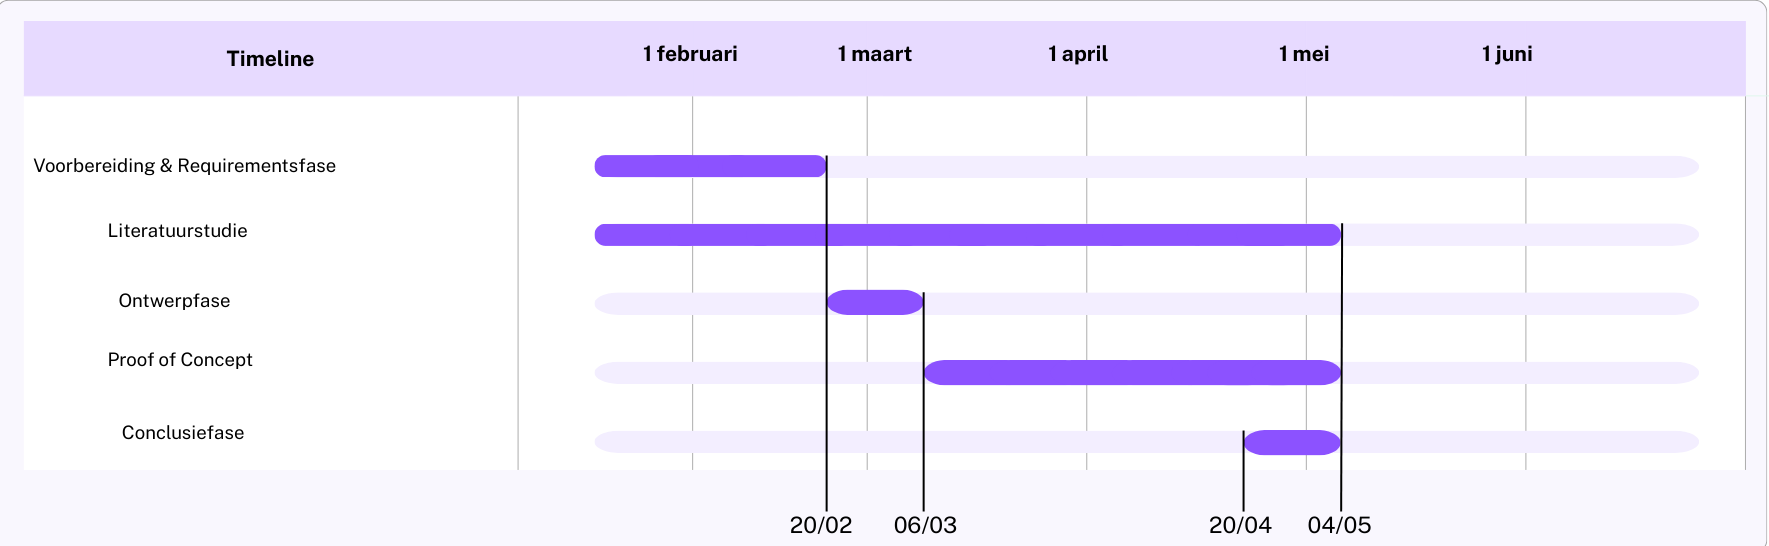
\includegraphics[width=.49\textwidth]{gantt_diagram.png}
%     \caption{Tijdslijn bachelorproef CRA-compliance via CI/CD-pijplijn.}
%     \label{fig:bp-tijdslijn}
% \end{figure}


% Voeg hier je eigen hoofdstukken toe die de ``corpus'' van je bachelorproef
% vormen. De structuur en titels hangen af van je eigen onderzoek. Je kan bv.
% elke fase in je onderzoek in een apart hoofdstuk bespreken.

%\input{...}
%\input{...}
%...

%%=============================================================================
%% Conclusie
%%=============================================================================

\chapter{Conclusie}%
\label{ch:conclusie}

% TODO: Trek een duidelijke conclusie, in de vorm van een antwoord op de
% onderzoeksvra(a)g(en). Wat was jouw bijdrage aan het onderzoeksdomein en
% hoe biedt dit meerwaarde aan het vakgebied/doelgroep? 
% Reflecteer kritisch over het resultaat. In Engelse teksten wordt deze sectie
% ``Discussion'' genoemd. Had je deze uitkomst verwacht? Zijn er zaken die nog
% niet duidelijk zijn?
% Heeft het onderzoek geleid tot nieuwe vragen die uitnodigen tot verder 
%onderzoek?

\section{Beantwoording van de onderzoeksvraag}

De centrale onderzoeksvraag van deze bachelorproef luidde: \enquote{Hoe kan een CI/CD-pipeline geautomatiseerd worden om CRA-compliant te zijn?} Deze vraag werd benaderd via een literatuurstudie over de Cyber Resilience Act, SBOMs, CVE-analyse en DevSecOps-praktijken, gecombineerd met een Proof of Concept in de context van Excentis.

Naast de centrale onderzoeksvraag worden ook een aantal deelvragen beantwoord. In het probleemdomein werd de Cyber Resilience Act toegelicht, werden de basisprincipes van CI/CD en DevSecOps besproken en werd de concrete impact voor Excentis in kaart gebracht. In het oplossingsdomein werd vervolgens onderzocht hoe een CI/CD-pipeline technisch kan worden opgebouwd, welke CRA-relevante securitycontroles geautomatiseerd kunnen worden, welke tools hiervoor beschikbaar zijn en welke technische en organisatorische uitdagingen daarbij optreden.

Op basis van de resultaten van de PoC kan geconcludeerd worden dat CRA-relevante securitycontroles in belangrijke mate geautomatiseerd kunnen worden binnen een CI/CD-pipeline. De ontwikkelde Jenkins-pipeline genereert een SBOM, \\voert dependency-scans, SAST, container image scanning, secrets scanning en DAST uit en archiveert de resultaten als auditbewijs. Kwetsbaarheden met een hoge CVSS-score blokkeren de pipeline via quality gates, waardoor releases met kritieke risico's niet ongemerkt kunnen doorglippen. Volledige CRA-compliance kan hiermee echter nog niet \emph{gegarandeerd} worden: er blijft een menselijke controle nodig voor onder meer het controleren van false positives, het beoordelen van contextafhankelijke risico's en het aanleveren van aanvullende gegevens zoals de SHA-512-hash van het deployable component in de SBOM.

\section{Belangrijkste bevindingen}

Een eerste belangrijke bevinding uit de literatuurstudie is dat de bouwstenen voor geautomatiseerde CRA-compliance in CI/CD-pipelines in grote mate reeds bestaan. Open source tools zoals Syft, OWASP Dependency-Check, Grype, SonarQube en OWASP ZAP dekken samen een groot deel van de vereiste controles, terwijl de CRA zelf vooral high-level verplichtingen formuleert en geen concreet technisch stappenplan oplegt. Tegelijk is er nog geen eenduidige, gestandaardiseerde aanpak om deze vereisten rechtstreeks naar de pipeline-stappen te vertalen.

Een tweede bevinding is dat de geïntegreerde Jenkins-pipeline in deze bachelorproef aantoont dat een combinatie van SBOM-generatie, SCA, SAST, container scanning, secrets scanning en DAST technisch haalbaar is zonder de bestaande ontwikkelworkflow fundamenteel te verstoren. De referentierun met Spring Petclinic toont dat de totale doorlooptijd (7 minuten en 28 seconden) aanvaardbaar blijft, terwijl meerdere kwetsbaarheden en validatieproblemen automatisch worden opgespoord en gerapporteerd.

Ten slotte blijkt uit de resultaten dat automatisering nooit alle complexiteit wegneemt. False positives, onvolledige of inconsistente CPE-data in kwetsbaarheidsdatabanken en de afweging tussen risico en businessimpact blijven domeinen waar menselijke expertise noodzakelijk is. De pipeline kan signaleren en blokkeren, maar iemand moet nog steeds bewuste beslissingen nemen over uitzonderingen en remediatie.

\section{Praktische meerwaarde voor Excentis}

Voor Excentis levert deze bachelorproef een concrete referentie-implementatie op waarmee het bedrijf de eerste stappen richting CRA-compliance kan zetten. De uitgewerkte Jenkins-pipeline sluit aan bij de bestaande tooling, maakt gebruik van uitsluitend open source componenten en toont hoe SBOM-generatie, kwetsbaarheidsscans en rapportage geïntegreerd kunnen worden in één geautomatiseerde workflow.

De pipeline biedt ontwikkelteams vroegtijdige feedback over kwetsbaarheden in code, dependencies en containerimages, terwijl management inzicht krijgt in de securitystatus via rapporten en archiveringsmechanismen. Daarmee beantwoordt de oplossing rechtstreeks aan de in de requirementsanalyse geformuleerde noden: tijd- en kostenbesparing door automatisering, systematische rapportering in plaats van ad-hoc-communicatie en een herbruikbaar framework dat op meerdere projecten kan worden toegepast.

\section{Beperkingen en toekomstig onderzoek}

Ondanks de positieve resultaten kent deze bachelorproef belangrijke beperkingen. De PoC is concreet uitgewerkt voor één Java-gebaseerde demo-applicatie en ontworpen om ook uitbreidbaar te zijn naar .NET- en Python-projecten met een geselecteerde set tools die eenvoudig in Jenkins te integreren zijn. Multi-repo-omgevingen, microservice-architecturen en complexe releaseketens werden niet onderzocht. De koppeling tussen SBOMs en CVE-databases is slechts gedeeltelijk geautomatiseerd: het valideren van SBOM-kwaliteit tegen BSI TR-03183-2 en het verrijken met onder meer hashwaarden vereist nog bijkomend werk.

Daarnaast blijft de menselijke factor cruciaal. False positives in SCA- en container-scanners, contextafhankelijke risico-inschattingen en het opstellen van organisatiebrede policies rond vulnerability-acceptatie en retentie van bewijsmateriaal kunnen niet louter aan tools worden overgelaten. Zonder duidelijke processen en verantwoordelijkheden bestaat het risico dat waarschuwingen genegeerd worden of dat rapporten niet structureel worden opgevolgd.

Tot slot roept dit onderzoek nieuwe vragen op over de keuze tussen een open source-gebaseerde aanpak en commerciële all-in-one-platformen zoals Snyk of Aikido Security, die in de literatuurstudie werden besproken. Open source tools bieden maximale controle, flexibiliteit en geen licentiekost, maar vragen meer integratie- en onderhoudsinspanning. Commerciële platforms kunnen daarentegen unified dashboards, betere prioritering en lagere false-positive-ratio's bieden, maar brengen licentiekosten en vendor lock-in met zich mee. Verdiepend onderzoek kan nagaan welk model, of welke hybride combinatie, op lange termijn het meest geschikt is voor een organisatie zoals Excentis.

Samengevat toont deze bachelorproef aan dat een CI/CD-pipeline een belangrijke hefboom kan zijn om CRA-compliance te ondersteunen, maar dat volledige naleving alleen bereikt wordt wanneer geautomatiseerde securitycontroles hand in hand gaan met duidelijke processen, menselijke expertise en weloverwogen technologische keuzes.


%---------- Bijlagen -----------------------------------------------------------

\appendix

\chapter{Onderzoeksvoorstel}

Het onderwerp van deze bachelorproef is gebaseerd op een onderzoeksvoorstel dat vooraf werd beoordeeld door de promotor. Dat voorstel is opgenomen in deze bijlage.

%% TODO: 
%\section*{Samenvatting}

% Kopieer en plak hier de samenvatting (abstract) van je onderzoeksvoorstel.

% Verwijzing naar het bestand met de inhoud van het onderzoeksvoorstel
%---------- Inleiding ---------------------------------------------------------

% Is dit voorstel gebaseerd op een paper van Research Methods die je
% vorig jaar hebt ingediend? Heb je daarbij eventueel samengewerkt met een
% andere student?
% Zo ja, haal dan de tekst hieronder uit commentaar en pas aan.

%\paragraph{Opmerking}

% Dit voorstel is gebaseerd op het onderzoeksvoorstel dat werd geschreven in het
% kader van het vak Research Methods dat ik (vorig/dit) academiejaar heb
% uitgewerkt (met medesturent VOORNAAM NAAM als mede-auteur).
% 

\section{Inleiding}%
\label{sec:inleiding}

Deze bachelorproef richt zich op het automatiseren van CRA-compliance aan de hand van\\CI/CD-pipelines binnen de softwareontwikkeling bij Excentis, een bedrijf dat netwerkhardware zoals de ByteBlower en XRA ontwikkelt en verkoopt. Door de invoering van de Europese Cyber Resilience Act (CRA) krijgen digitale producten striktere cybersecurity verplichtingen \parencite{EU_CRA}. Hierdoor moet software tegen december 2027 voldoen aan de vereisten van de CRA wetgeving om een CE-label te verkrijgen \parencite{EuropeanCommission2024CRAnews}. \begin{tcolorbox}[colback=probkleur, colframe=probkleur, boxrule=0pt, sharp corners, enhanced, breakable]Dit betekent dat de software die door Excentis wordt ontwikkeld conform moet zijn met deze wetgeving. Dit is dus een grote uitdaging voor zowel development teams als management teams. Volgens \textcite{Robyn2025} verwachten de klanten dat Excentis hier ook expliciet mee aan de slag gaat, waardoor het probleem een concrete en bedrijfsrelevante casus vormt. Dit verzekert niet alleen CRA-compliance, maar het ondersteunt ook het klantenvertrouwen, waardoor de producten veilig en op tijd op de markt kunnen worden gebracht.\end{tcolorbox}

Het doel van de bachelorproef is het ontwerpen en implementeren van een volledige CI/CD-pipeline die automatisch de CRA-compliance van de software controleert. Hierdoor zal het onderzoek ook een concrete oplossing bieden voor de specifieke probleemsituatie van Excentis, namelijk het waarborgen van veilige en CRA-compliant software, binnen de gestelde deadlines van de CRA. De gemaakte pipeline zal dienen als een Proof of Concept en laat Excentis toe om kwetsbaarheden te vinden, een Software Bill of Materials (SBOM) te genereren en hiertegen CVE-scans uit te voeren, waarbij er automatisch een rapportage plaatsvindt naar de betrokken development en management teams. 

De centrale onderzoeksvraag is dan ook: Hoe kan een CI/CD-pipeline geautomatiseerd worden om CRA-compliant te zijn? Het verwachte eindresultaat van deze bachelorproef is dan ook een werkende CI/CD-pipeline die voldoet aan de vereisten van Excentis. Aangezien dit onderzoek expliciet gericht is op Excentis en hun interne teams, is deze oplossing goed afgebakend en direct toepasbaar binnen de bedrijfscontext.


%---------- Stand van zaken ---------------------------------------------------

\section{Literatuurstudie}%
\label{sec:literatuurstudie}
\begin{tcolorbox}[
  colback=probleemdomein,
  colframe=probleemdomein,
  boxrule=0pt,
  sharp corners,
  enhanced,
  breakable
]
In deze literatuurstudie proberen we een antwoord te vinden op de volgende onderzoeksvragen binnen het probleemdomein:
\begin{itemize}
  \item Wat is de Cyber Resilience Act (CRA), en welke doelstellingen en verplichtingen bevat het?
  \item Wat is CI/CD en waarom is dit belangrijk binnen DevOps?
  \item Wat is de impact van CRA voor Excentis, welke producten worden getroffen en wat zien zij als verwachte output?
\end{itemize}
\end{tcolorbox}
\begin{tcolorbox}[
  colback=oplossingsdomein,
  colframe=oplossingsdomein,
  boxrule=0pt,
  sharp corners,
  enhanced,
  breakable
]
Daarnaast worden ook de onderzoeksvragen uit het oplossingsdomein behandeld:
\begin{itemize}
  \item Hoe wordt een CI/CD-pipeline technisch opgebouwd binnen een DevOps-omgeving en welke voordelen biedt automatisatie voor beheer en beveiliging?
  \item Hoe kunnen beveiligingscontroles en compliancevereisten uit de Cyber Resilience Act geïntegreerd en geautomatiseerd worden binnen CI/CD-pipelines, inclusief welke\\CRA-vereiste securitycontroles geautomatiseerd moeten worden en welke software bestaat om een SBOM te genereren?
  \item Welke technische en organisatorische uitdagingen kunnen optreden bij het automatiseren van CRA-compliance in CI/CD-pipelines?
\end{itemize}
\end{tcolorbox}
\subsection{Inleiding}

Er is de voorbije jaren sterke evolutie geweest in onderzoek naar de automatisering van beveiligingstesten om gevaarlijke commits op te sporen en security-scans te integreren in het ontwikkelingsproces. Omdat de complexiteit van software steeds toeneemt en\\supply-chain-aanvallen groeien, richten steeds meer bedrijven zich op DevSecOps, waarbij beveiliging vanaf het begin in de CI/CD-pipeline wordt geïntegreerd \parencite{Takahashi2025}. Ondertussen verplicht de nieuwe Europese wetgeving, zoals de Cyber Resilience Act, fabrikanten van software- en hardwareproducten om hun producten duidelijk veilig en betrouwbaar te maken vóór deze op de markt komen \parencite{EU_CRA}. Deze literatuurstudie schetst de huidige stand van zaken rond CRA-compliance, beveiligingsautomatisering, SBOM-generatie en CVE-analyse, en toont welke problemen er vandaag nog bestaan.

De Cyber Resilience Act (CRA), die in 2024 in werking trad, is een Europese wetgeving die de cybersecurity van digitale producten verplicht stelt vóór deze op de markt komen \parencite{EU_CRA}. Het doel hiervan is het verbeteren van de digitale weerbaarheid van producten en het verkleinen van de risico’s door kwetsbaarheden in software en hardware op tijd te detecteren en mitigeren. Belangrijke verplichtingen van CRA bevatten onder andere: Security-by-design, Software Bill of Materials (SBOM), incidentrapportage en beveiligingsupdates en het uitrollen van patches.

De nieuwe wetgeving zorgt voor zowel kansen als uitdagingen voor organisaties. Langs de ene kant stimuleert het innovatie en meer cyberveiligheid waardoor ook de betrouwbaarheid van de producten verhoogt, maar langs de andere kant bestaat er ook onduidelijkheid over specifieke productcategoriën, interpretatie van vereisten en implementatietijdlijnen van 36 maanden \parencite{ECSO2024}.\\Deze wetgeving is dan ook cruciaal voor bedrijven zoals Excentis, aangezien dat de naleving bepaalt of het product in aanmerking komt voor een CE-certificering \parencite{EuropeanCommission2024CRAnews}.

\subsection{CI/CD en DevSecOps}

Continuous Integration (CI) en Continuous Delivery/Deployment (CD) is een manier om software sneller en betrouwbaarder te ontwikkelen. Dit staat voor het continue en automatische integratie van code door developers en het continue leveren en/of deployen van deze code door een operations team \parencite{RedHat2025}.

Er wordt binnen de CI/CD-omgeving steeds vaker DevSecOps toegepast, waarbij beveiliging vanaf het begin in de ontwikkelingscyclus wordt geïntegreerd \parencite{RamdassJain2025}. DevSecOps is een evolutie van de originele DevOps waar ook Security een centraal onderdeel wordt. Dit wil dus zeggen dat beveiligingstesten zoals Static Application Security Testing (SAST) en Dynamic Application Security Testing (DAST) automatisch uitgevoerd zullen worden in de CI/CD-pipeline \parencite{Singh2025, Patel2024}. Dankzij deze extra stap kunnen kwetsbaarheden opgespoord en opgelost worden voordat deze code in productie gebruikt zal worden. Dit vermindert dan ook de kans op ernstige beveiligingsincidenten waardoor het product direct beter voldoet aan CRA-vereisten.

Ook maakt de automatisering binnen CI/CD-pipelines het mogelijk om beveiligingscontroles en compliance continu te monitoren. Dankzij tools die SBOMs genereren en CVE-scans uitvoeren ontstaat een end-to-end workflow die zowel kwaliteit als veiligheid van de software kan ondersteunen \parencite{OpenSSF2025SBOMCRA, Cheenepalli2025}. Voor organisaties zoals Excentis betekent dit dat CRA-compliance proactief kan worden afgedwongen, terwijl de ontwikkelsnelheid en productiviteit behouden blijven.

\subsection{Open vragen}

Uit recente literatuur blijkt dat er veel vooruitgang is in beveiligingsautomatisatie binnen CI/CD-omgevingen. Ondanks deze vooruitgang zijn er nog verschillende open vragen binnen het domein van CRA-compliance. Eén van de belangrijkste open vragen is dat er geen eenduidige richtlijn over hoe de CRA-vereisten technisch moeten worden vertaald binnen CI/CD-pipelines, zoals verplichte stappen, het type rapporten of validatieregels. Verschillende studies beschrijven wel de nood aan automatisering binnen DevSecOps \parencite{Singh2025,RamdassJain2025}, maar omdat de CRA zo recent is, bestaat er nog geen kant-en-klare oplossing.

Ook tonen bestaande DevSecOps-publicaties aan dat beveiliging steeds vaker geautomatiseerd wordt in CI/CD-pipelines \parencite{Singh2025,RamdassJain2025}. Deze literatuur richt zich voornamelijk op algemene softwarebeveiliging en niet specifiek op CRA-naleving. Er is dus nog onvoldoende onderzocht welke tools en workflows het best geschikt zijn om CRA-compliance te ondersteunen.

Tot slot is er ook veel onduidelijkheid over de operationele haalbaarheid. Organisaties willen voldoen aan de vereisten van CRA om zo een CE-label te behalen, wat vaak aanzienlijke tijd en middelen kost. Er is iemand nodig om dit te implementeren en opvolgen, en die persoon moet dan ook goed snappen hoe de CRA wetgeving in elkaar zit. Aangezien dat deze wetgeving splinternieuw is, is het ook moeilijk om iemand te vinden die zich hier in specialiseert.

Samengevat toont deze state-of-the-art dat er veel vooruitgang geboekt is op het vlak van CI/CD-pipelines maar dat er wel nog een lange weg te gaan is, zeker omtrent de CRA-wetgeving.


% Voor literatuurverwijzingen zijn er twee belangrijke commando's:
% \autocite{KEY} => (Auteur, jaartal) Gebruik dit als de naam van de auteur
%   geen onderdeel is van de zin.
% \textcite{KEY} => Auteur (jaartal)  Gebruik dit als de auteursnaam wel een
%   functie heeft in de zin (bv. ``Uit onderzoek door Doll & Hill (1954) bleek
%   ...'')


%---------- Methodologie ------------------------------------------------------
\section{Methodologie}%
\label{sec:methodologie}

Het onderzoek van deze bachelorproef zal worden uitgevoerd in een technische en toegepaste context bij het bedrijf Excentis, met als focus het automatiseren van CRA-compliance aan de hand van CI/CD-pipelines. Dit onderzoek zal in verschillende fases verlopen, waarbij elke fase een duidelijk doel, resultaat alsook een deadline heeft. 

De eerste fase is de voorbereiding en requirementsfase. Hierbij wordt de huidige status van pipelines bij Excentis in kaart gebracht. Dit zal gebeuren aan de hand van gesprekken met de co-promotor en indien nodig andere relevante werknemers. In deze fase zal er vooral informatie verzameld worden over welke software Excentis gebruikt voor de pipelines (zoals GitHub Actions, Jenkins,…), en de securityvereisten vanuit de CRA-wetgeving en het bedrijf zelf. Het doel van deze fase is om op voorhand goed te weten waar er aan begonnen wordt. De deadline hiervoor is 20 februari. 

De volgende fase is de literatuurstudie, dit zal tegelijkertijd lopen met alle andere fases aangezien dit begint bij de start van het onderzoek en pas eindigt op het einde van het onderzoek. In deze fase worden alle theoretische onderwerpen onderzocht, zoals de Cyber Resilience Act, best practices voor CI/CD-pipelines, geautomatiseerde securitytesten, SBOM-generatie en CVE-analyse. Het doel van deze fase is om alle theoretische onderwerpen die aan bod komen goed te begrijpen en uit te leggen. De deadline hiervoor is 4 mei. 

Hierna is de ontwerpfase. In deze fase zal de CI/CD-pipeline op basis van alle verzamelde informatie en kennis ontworpen worden. Hier zal een lijst met benodigde tools geselecteerd worden, zoals BurpSuite, Aikido, Snyk,... en de workflow van de pipeline zal ook hier gedefinieerd worden. Ook wordt er hier een shortlist aan extra securitytesten gemaakt die zullen uitgevoerd worden in de pipeline. Ook wordt er hier gekeken naar al bestaande opties voor SBOM-generatie en CVE-scans, en indien nodig ook een ontwerp om zelf een SBOM te genereren. Het doel is hier om een goede workflow te hebben van wat allemaal nog gedaan zal moeten worden tijdens de Proof of Concept fase. De deadline hiervoor is 6 maart. 

De voorlaatste fase is de Proof of Concept fase. Hier wordt de CI/CD-pipeline effectief gemaakt, grondig getest en op punt gesteld met voorbeeldcode. Hoe het in elkaar zal zitten zal afhangen van alle andere vorige fases. Afhankelijk van de requirements van Excentis zelf, de verwachtingen van de CRA, en de beste tools voor automatische testen, welke tools maken goede en makkelijke SBOM’s,… Het doel van deze fase is het ontwikkelen van een werkende pipeline die automatisch de code test op CRA-compliance. De deadline voor dit is ook 4 mei. 

De laatste fase is de conclusiefase. Hier gaat er vermeld worden of de Proof of Concept volledig uitgewerkt is kunnen worden, of alles gewerkt heeft en of Excentis dit een succes beschouwt. De deadline voor deze fase is nogmaals 4 mei en het doel hiervan is om te zien of deze bachelorproef tot een goed einde is gebracht.

\begin{figure}[h]
    \centering
    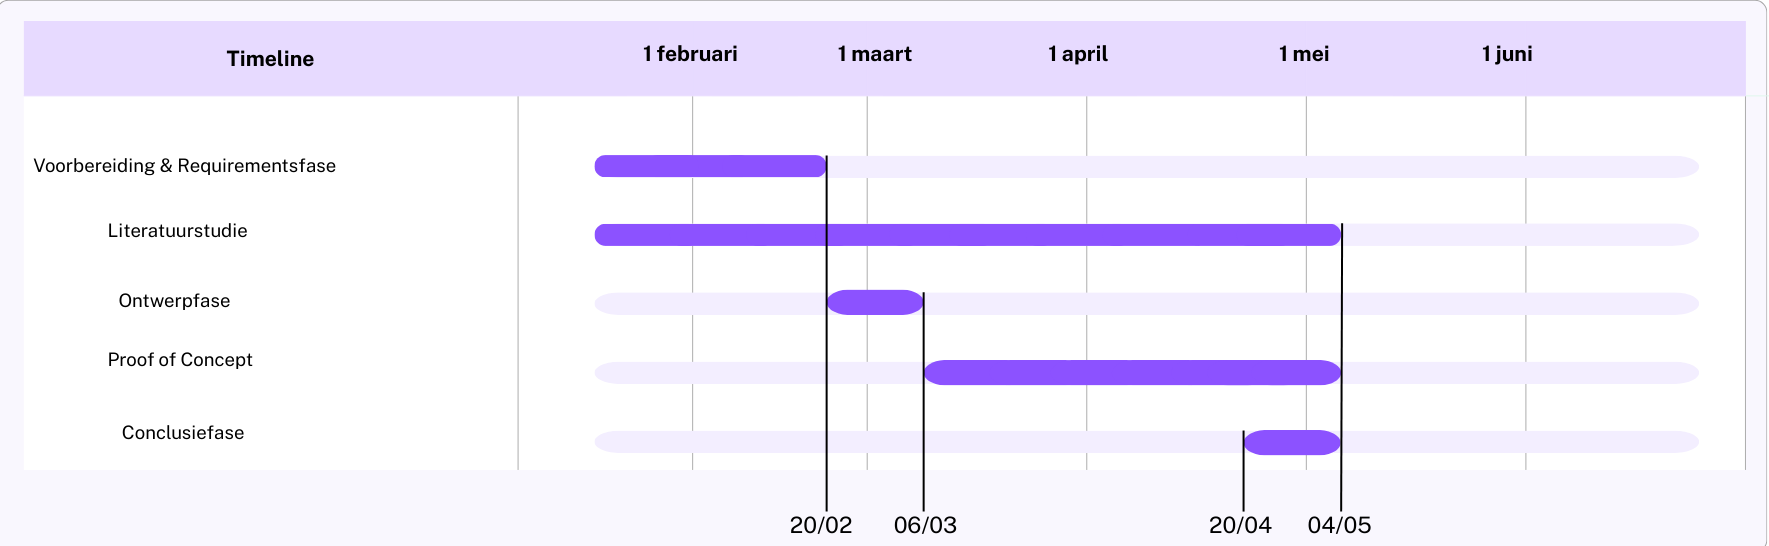
\includegraphics[width=.49\textwidth]{gantt_diagram.png}
    \caption{Tijdslijn bachelorproef CRA-compliance via CI/CD-pijplijn.}
    \label{fig:bp-tijdslijn}
\end{figure}
%---------- Verwachte resultaten ----------------------------------------------
\section{Verwacht resultaat, conclusie}%
\label{sec:verwachte_resultaten}

Het verwachte resultaat van deze bachelorproef is een volledig werkende CI/CD-pipeline die alle nodige securitytesten uit de shortlist uitvoert en een SBOM maakt en deze vergelijkt met een CVE-database waardoor de code volledig CRA-compliant is. Dit zorgt ervoor dat bekende en onbekende kwetsbaarheden opgespoord kunnen worden en gerapporteerd worden aan het development team zodat zij deze zo snel mogelijk kunnen oplossen. Hierdoor kan Excentis sneller en efficiënter inspelen op security-risico’s en wordt de kans verhoogd dat hun software tijdig voldoet aan de vereisten van de Cyber Resilience Act, waardoor ze een CE-label kunnen verkrijgen.

Deze bachelorproef biedt een meerwaarde voor zowel de development teams als het management team van Excentis. Voor de developers maakt het vinden van kwetsbaarheden eenvoudiger en sneller. Tegelijkertijd krijgt het management team inzicht in de algemene compliance-status van de softwareproducten.

Hoewel het doel is om een volledig werkende CI/CD-pipeline te hebben, kunnen er zich altijd problemen ontstaan. Bijvoorbeeld, bepaalde securitytools of SBOM-generators kunnen beperkingen hebben die de automatisatie voor een deel beïnvloeden. Mocht dit gebeuren, wordt er een duidelijke motivatie gegeven waarom de oorspronkelijke verwachtingen niet volledig overeenkomen met de gerealiseerde resultaten.



%%---------- Andere bijlagen --------------------------------------------------
% TODO: Voeg hier eventuele andere bijlagen toe. Bv. als je deze BP voor de
% tweede keer indient, een overzicht van de verbeteringen t.o.v. het origineel.
%\input{...}

%%---------- Backmatter, referentielijst ---------------------------------------

\backmatter{}

\setlength\bibitemsep{2pt} %% Add Some space between the bibliograpy entries
\printbibliography[heading=bibintoc]

\end{document}
